\setcounter{secnumdepth}{-1}

\chapter{Synchronization errors}

\section{Description}

Because the receiver and transmitter are not at the same location, the carrier frequencies and the samplers at TX and RX will have a different phase and due to the inaccuracies of the oscillator, the frequencies will also be slightly different. \\
This is summarized in 4 effects:
\begin{itemize}
    \item \textbf{Carrier frequency offset (CFO)}: The difference in the carrier frequencies at TX and RX ($=\Delta \omega$). It will add ISI as the RRC are not anymore matched and a linearly increasing phase shift will appear.
    \item \textbf{Phase offset}: The difference between the phase of the carrier signal at TX and RX.
    \item \textbf{Sampling frequency offset (SFO)}: The difference in the sampling frequencies at TX and RX.
    \item \textbf{Time shift}: The difference in the timing of the samples at TX and RX.
\end{itemize}

\section{Implementation}

\subsection{CFO}
The CFO implementation is done by multiplying the signal with a complex exponential $e^{j2\pi \phi_{\text{ppm}}f_c t}$. The phase offset is added to the CFO. It is defined in ppm (part per million) where the ppm value is $\frac{\Delta\omega}{f_c} 10^{-6}$. \\
Figure \ref{fig:CFO_BER} shows the BER curves with different CFO values. In order to have useful results, the linear phase shift is removed right after the second RRC filter. This allows to only keep the effect of ISI on the BER curve.

\begin{figure}[H]
    \centering
    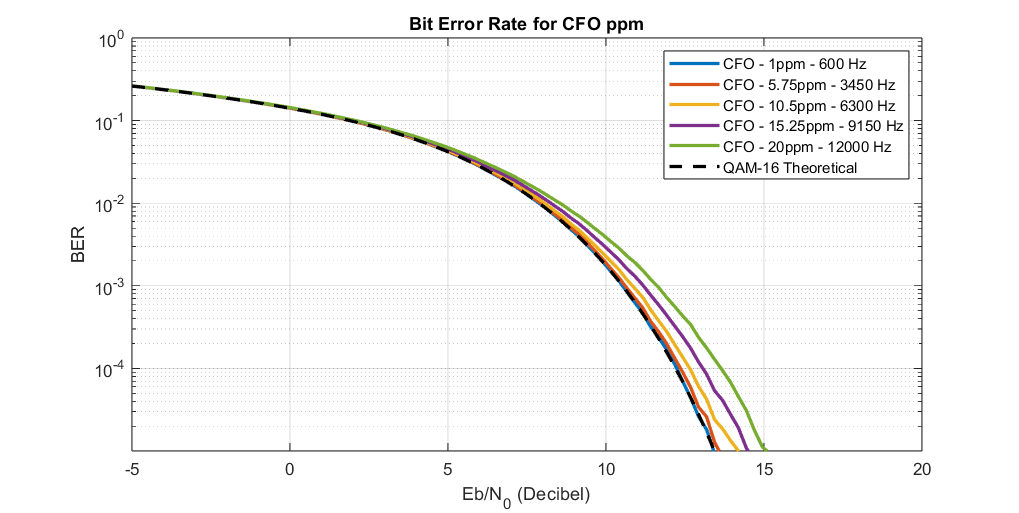
\includegraphics[width=0.8\textwidth]{CFO_ppm.png}
    \caption{BER with different CFO values}
    \label{fig:CFO_BER}
\end{figure}

Figure \ref{fig:CFO_const} shows the effect of CFO on the symbol constellation for QAM-16. It is here plotted without any noise and with parameters that allow us to see the line phase shift of the symbols. \\

\begin{figure}[H]
    \centering
    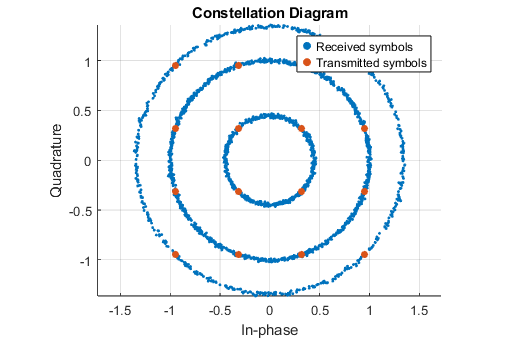
\includegraphics[width=0.8\textwidth]{constellation_CFO.png}
    \caption{Constellation before and after CFO}
    \label{fig:CFO_const}
\end{figure}

\subsection{Phase offset}
The same is done for the phase offset where the exponential is simply $e^{j\phi}$ where $\phi$ is chosen once at the begining of the simulation. \\

The effect of the phase offset is only visible on the constellation plot (figure \ref{fig:phaseOffsetConst}) where every point is rotated by a fixed angle (whereas CFO rotated the symbols linearly with time). \\

\begin{figure}[H]
    \centering
    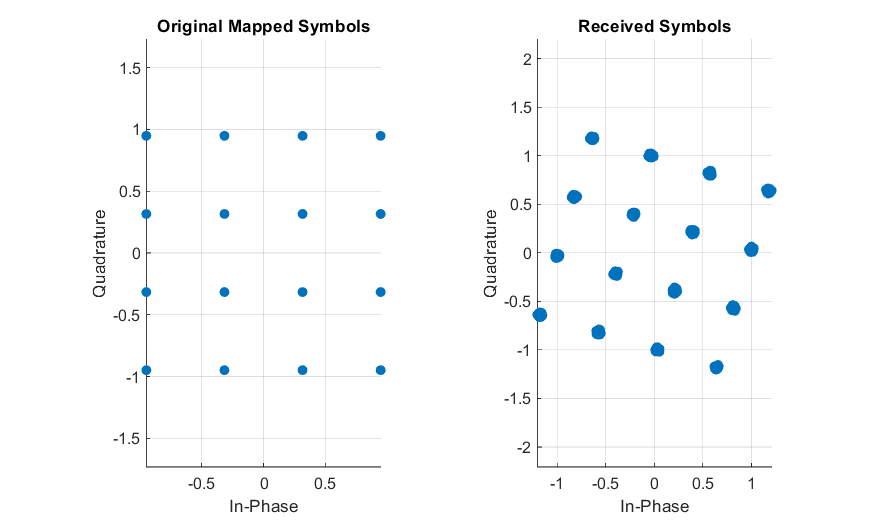
\includegraphics[width=0.8\textwidth]{constellation_carrier_offset.png}
    \caption{Constellation before and after phase offset}
    \label{fig:phaseOffsetConst}
\end{figure}

\subsection{SFO}
The SFO is neglected in the simulation as it would need some interpolation and more complex computations. \\
\subsection{Time shift}
The time shift is implemented by simply shifting the samples in the array with an oversampling factor that is large enough. \\

\section{Correction}


